\begin{quote}
    \textit{``If you're going to try to violate decoupling, don't try to do it with something as stupid as continuous functions.''
    ``Bastards.''
    ``That's correct.''
    }
    
    ---Nemanja Kaloper and Mark Samuel Abbott
\end{quote}

Last time, we found the explicit formula for the partial sums of a Fourier series to be
\begin{equation}
    f_N(x) = \frac{1}{2\pi} \int_{-\pi}^\pi dt\, f(t) \bkt{\frac{\sin((N+1/2)(x-t))}{\sin \frac{x-t}{2}}}.
\end{equation}
Let us consider a Heaviside step function,
\begin{equation}
    f(x) = \frac{h}{2}(2\Theta(x) - 1).
\end{equation}
    We found the Fourier series to be
\begin{equation}
    f(x) = \frac{2h}{\pi} \sum_{n=0}^\infty \frac{\sin \bkt{(2n+1)x}}{2n+1},
\end{equation}
and we'd like to study what happens when the sum is finite rather than infinite. That is, let us plug in $f(t)$. Then
\begin{align}
    f_N(x) &= \frac{1}{2\pi} \int_{-\pi}^\pi dt \paren{\frac{h}{2}(2\Theta(t) - 1)} \bkt{\frac{\sin((N+1/2)(x-t))}{\sin \frac{x-t}{2}}}\\
    &= \frac{h}{4\pi} \bkt{-\int_{-\pi}^0 dt \frac{\sin((N+1/2)(x-t))}{\sin \bkt{\frac{x-t}{2}}} + \int_0^\pi dt \frac{\sin((N+1/2)(x-t))}{\sin\bkt{\frac{x-t}{2}}}}.
    \label{eqn:fourierpartialsums}
\end{align}
Since this is a finite series and the function is piecewise continuous, we can now %manipulate the partial sums and exchange order of integration and summation as we like, then
take the limit of the interpolating functions $\lim_{N\to \infty}f_N(x)$ to get the infinite sum.


Note that
\begin{equation}
    \frac{1}{2\pi} \int_{-\pi}^\pi dt \frac{\sin \bkt{(N+1/2)(x-t)}} {\sin\bkt{\frac{x-t}{2}}} = 1.
\end{equation}
This is just the integral of (the limiting series of) a delta function. Why? This was just the sum
\begin{equation}
    \sum_{n=-N}^N e^{in(x-t)} = \frac{1}{2\pi}\frac{\sin \bkt{(N+1/2)(x-t)}}{\sin\bkt{\frac{x-t}{2}}},
\end{equation}
and if we integrate the LHS from $-\pi$ to $\pi$, then we have
\begin{equation}
    \int_{-\pi}^\pi dt \sum_{n=-N}^N e^{in(x-t)} = \sum_{n=-N}^N e^{inx} \int_{-\pi}^\pi dt \,e^{-int} = \sum_{n=-N}^N e^{inx} \paren{2\pi \delta_{n,0}},
\end{equation}
so the other terms in the sum drop out.
%If you're going to try to violate decoupling, don't try to do it with something as stupid as continuous functions.
%Bastards.
%That's correct.
%Did you like the diffraction grating problem on the prelim? With the path difference? That was mine. It is simple. But it is tricky.
% Note that our integral is not over a whole period. The behavior of the integral is under $t\to -t$, so for generic $x$, this function will be neither odd nor even.

We can rewrite the terms in our integrals \eqref{eqn:fourierpartialsums} in terms of new variables $-s=x-t$ in the first integral and $s=x-t$ in the second integral
to write
\begin{align*}
    f_N(x) &= \frac{h}{4\pi} \bkt{-\int_{-\pi}^0 dt \frac{\sin((N+1/2)(x-t))}{\sin \bkt{\frac{x-t}{2}}} + \int_0^\pi dt \frac{\sin((N+1/2)(x-t))}{\sin\bkt{ \frac{x-t}{2}}}}\\
        &= \frac{h}{\pi} \bkt{-\int_{-\pi-x}^{-x} ds \frac{\sin((N+1/2)(-s))}{\sin \bkt{\frac{-s}{2}}} - \int_{x}^{-\pi+x} ds \frac{\sin((N+1/2)s)}{\sin\bkt{ \frac{s}{2}}}}\\
        &=\frac{h}{4\pi} \bkt{-\int_{-\pi-x}^{-x} ds \frac{\sin((N+1/2)s)}{\sin \bkt{\frac{s}{2}}} + \int_{-\pi+x}^{x} ds \frac{\sin((N+1/2)s)}{\sin\bkt{ \frac{s}{2}}}}\numberthis\label{eqn:integrationlimits_preshuffle}
%&=\frac{h}{4\pi} \bkt{+\int_{-\pi+x}^{+x} ds \frac{\sin((N+1/2)s)}{\sin \bkt{\frac{s}{2}}} - \int_{-\pi - x}^{-x} ds \frac{\sin((N+1/2)(s))}{\sin\bkt{ \frac{s}{2}}}}.
% &= \frac{h}{\pi} \bkt{-\int_{-\pi+x}^{+x} ds \frac{\sin((N+1/2)(-s))}{\sin \bkt{\frac{-s}{2}}} + \int_{-x}^{\pi-x} ds \frac{\sin((N+1/2)(-s))}{\sin\bkt{ \frac{-s}{2}}}}\\
% &=\frac{h}{4\pi} \bkt{-\int_{-\pi+x}^{+x} ds \frac{\sin((N+1/2)s)}{\sin \bkt{\frac{s}{2}}} + \int_{-x}^{\pi-x} ds \frac{\sin((N+1/2)(s))}{\sin\bkt{ \frac{s}{2}}}}\\
% &=\frac{h}{4\pi} \bkt{+\int_{-\pi+x}^{+x} ds \frac{\sin((N+1/2)s)}{\sin \bkt{\frac{s}{2}}} - \int_{-\pi - x}^{-x} ds \frac{\sin((N+1/2)(s))}{\sin\bkt{ \frac{s}{2}}}}.
\end{align*}
\begin{figure}
    \centering
    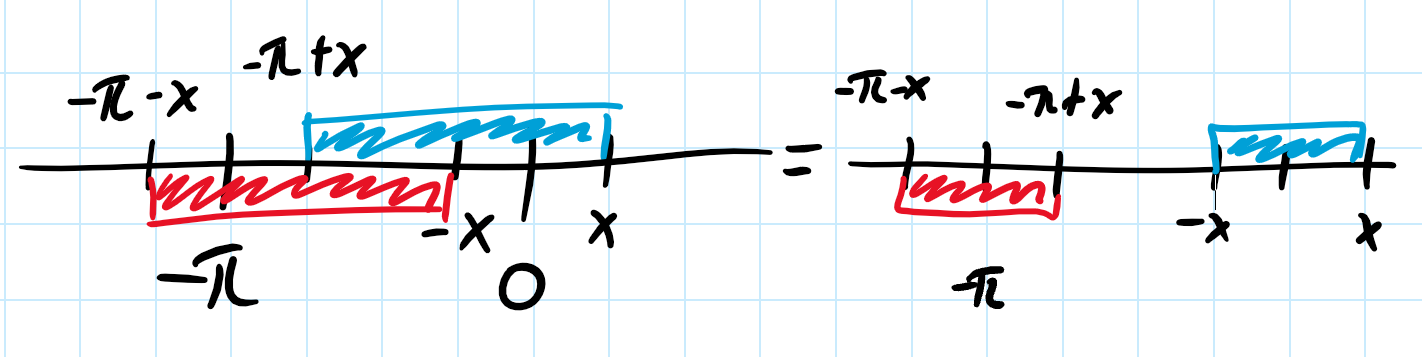
\includegraphics[width=0.75\textwidth]{2020/01/20200117_integrationlimits.PNG}
    \caption{An illustration of how to rewrite the integration limits in Eqn.~\eqref{eqn:integrationlimits_preshuffle}.}
    \label{fig:integrationlimits}
\end{figure}
Let's justify the signs here. There are two sign flips on the second term. One comes from $ds = -dt$, while the other comes from exchanging the limits of integration in the third line. There are no sign flips on the first term, since 
\begin{gather*}
    \sin((N+1/2)(-s) = -\sin((N+1/2)s), \quad\sin(-s/2) = -\sin(s/2)\\ 
    \implies \frac{\sin((N+1/2)(-s)}{\sin(-s/2)} = \frac{\sin((N+1/2)s)}{\sin(s/2)}.
\end{gather*}

We can now shuffle the limits of integration in Eqn.~\eqref{eqn:integrationlimits_preshuffle} a bit (see Fig.~\ref{fig:integrationlimits}) to get
\begin{equation}
    f_N(x) = \frac{h}{4\pi}\bkt{+\int_{-x}^{+x} ds \frac{\sin((N+1/2)s)}{\sin \bkt{\frac{s}{2}}} - \int_{-\pi - x}^{-\pi + x} ds \frac{\sin((N+1/2)s)}{\sin\bkt{ \frac{s}{2}}}}.\label{eqn:fourier_newlimits}
\end{equation}
One way to do this formally is to recognize that the relative sign between these two integrals allows us to rewrite the definite integrals as differences of indefinite integrals (denoted $\Phi$):
\begin{align*}
    -\int_{-\pi-x}^{-x} f(x) dx +\int_{-\pi+x}^x f(x)dx &= -\bkt{\Phi(-x) - \Phi(-\pi - x)} + \bkt{\Phi(x) - \Phi(-\pi +x)}\\
        &= (\Phi(x)-\Phi(-x)) - (\Phi(-\pi+x) - \Phi(-\pi -x))\\
        &= \int_{-x}^x f(x) dx -\int_{-\pi-x}^{-\pi +x} f(x) dx.
\end{align*}
Graphically or otherwise, we arrive at the result~\eqref{eqn:fourier_newlimits}.

Now what happens as $x\to 0$? Our integration measure $ds$ gets vanishingly small, and if the integrand were finite on that range, the integral would vanish. Well, the second term, the integral on an interval around $-\pi$, is bounded, since $\sin((N+1/2)s)$ is bounded around $s=-\pi$, and the denominator 
\begin{equation*}
    \lim_{s\to -\pi} \sin(s/2) =\sin(-\pi/2)=-1
\end{equation*}
is perfectly well-behaved. So indeed the second integral in \eqref{eqn:fourier_newlimits} is zero. More precisely, it is proportional to the interval length $2x$, which goes to zero as $x\to 0$.

The first term is different. We are taking an integral in a region around $s=0$, but $\sin(0)$ is zero, so the denominator will cause the integrand to diverge as $s\to 0$. The numerator $\sin((n+1/2)s)$ also goes to zero, so we get an indeterminate ratio which we can work out with L'H\^opital's rule or equivalently by Taylor expansion around $s=0$. That is,
\begin{equation}
    \lim_{x\to 0} \frac{h}{4\pi} \int_{-x}^x \frac{\sin((N+1/2)s)}{\sin(s/2)} ds = \lim_{x\to 0} \frac{h}{4\pi} \int_{-x}^x ds \frac{(N+1/2)s}{(s/2)} = \lim_{x\to 0} \frac{h}{2\pi} \int_{-x}^x ds (N+1/2)  
\end{equation}
%
The factors of $s$ have cancelled. Now we must be careful about the order of limits. If we hold $N$ fixed and perform the $ds$ integral, then we get
\begin{equation}
    \lim_{x\to 0} f_N(x) = \lim_{x\to 0} \frac{h}{2\pi}(N+1/2)(2x) = 0.
\end{equation}
It follows that
\begin{equation}
    f_N(0) = 0 \implies f(0) = \lim_{N\to \infty} f_N(0) =  0.
\end{equation}
%But then all the functions in the series are zero, which tells us that the value of the step function is the limit as $N\to \infty$ after $x\to 0$, i.e.
That is, the (shifted) step function takes on the value
\begin{equation}
    f(0) = \Theta(0)-1/2=0 \implies \Theta(0) = \frac{1}{2},
\end{equation}
the average of its value on either side of $x=0$.

Moreover, if we look at the Fourier series approximation of the step function, we find that the approximation overshoots the step. This is called the \term{Gibbs phenomenon}. Curiously, the overshoot doesn't improve with more terms; in fact, it approaches a limiting value of about $18\%$. The reason for this is simply that we're trying to approximate a discontinuous function with a smooth one. We overshoot because the derivative cannot change too quickly. Next time, we will study the behavior of
\begin{equation}
    \frac{h}{2\pi} \int_0^x \frac{\sin\bkt{(N+1/2)s}{\sin(s/2)}} dx,
\end{equation}
and we can study the behavior of this integral in terms of a new variable
\begin{equation}
    \zeta = (N+\frac{1}{2})s.
\end{equation}
Then we have an integral
\begin{equation}
    \frac{h}{2\pi} \int_0^{(N+1/2)x} \frac{\sin(\zeta)}{\sin(\zeta/(2N+1))} d\zeta \approx \frac{h(2N+1)}{2\pi} 
    \frac{h}{2\pi} \int_0^{(N+1/2)x} \frac{\sin(\zeta)}{\zeta} d\zeta
\end{equation}
and we can study this in certain limits of $\zeta$.